\subsection{Approach Overview}


\begin{figure}[t]
	\begin{center}
		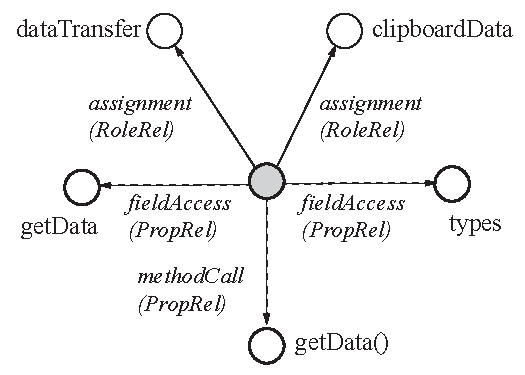
\includegraphics[width=.7\columnwidth]{figures/stargraph.pdf}
		\caption{Training Process}
		\label{training_process}
	\end{center}
\end{figure}

\begin{figure}[t]
	\begin{center}
		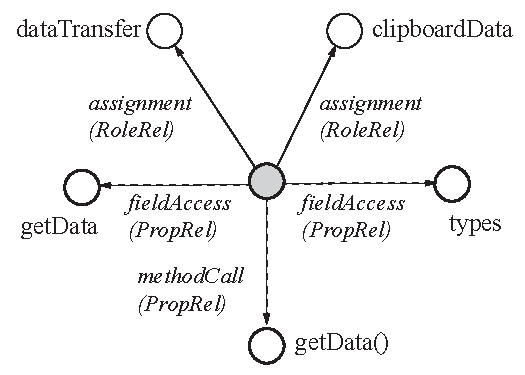
\includegraphics[width=.7\columnwidth]{figures/stargraph.pdf}
		\caption{Testing Process}
		\label{testing_process}
	\end{center}
\end{figure}

Step 1. Generate graphs...

Step 2. Variable Type Generation:
1> Graph edge represent different relations (This may change depends on the graph we finally want to use). Each node is a variable, method call, or a field of an object. We use the name of the variable (minified), method call, or the field as the node feature and use GloVe to learn the representation vector.
2> We use EGCN that accepts graphs with both node features and edges features as input. Here the edge feature is the edge type. 
3> The output of EGCN is the generated representation vector $V_r$ for each node. 
4> We combined the representation vector we get from EGCN with the generated from the next step $V'_r$ (variable name generation) by using the cross-product and get the final generated representation vector for type prediction ($V_f$)
5> We use a GRU (RNN) as decoder accepts the $V_f$ as input and generates the type for the variables as output.
6> When generating the type, we use some basic rule from parser to reduce the possible candidates.

Step 3. Variable Name Generation:
1> Similar to step 2, we use GloVe to learn the representation vector.
2> For the node that represent the variable with minified name, we mask the node feature and regard it as the missing feature.
3> Put the graph with missing feature for some nodes into the $GCN_{mf}$ as input. 
4> The $GCN_{mf}$ can output the predicted missing node feature representation vector $V_{rm}$ and the node representation vector $V'_r$. The node representation vector $V'_r$ will be used in step 2.
5> Use $V_{rm}$ as the input of a GRU (RNN) decoder, and the decoder generate the names for the variables with the minified name.
6> When doing generation, we apply basic checking to make sure the same variable has only one consistent name.

Step 4. Multi-task learning
We use the uncertainty weighted multi-task loss as the multitask learning loss function and use the maximum of the top-1 accuracy score from two tasks as the training target.
 